
\section{Wallis' slow road to $\pi$}

Wallis' formula is an infinite product that converges (slowly) to
$\pi$:\begin{equation}
\pi=\prod_{i=1}^{\infty}\frac{4i^{2}}{4i^{2}-1}.\end{equation}


The listing~\ref{code:wallis_pi} contains a skeleton with no
implementation but with some plotting commands already inserted, so
that you can visualize the convergence rate of this formula as more
terms are kept.

\lstinputlisting[label=code:wallis_pi,caption={IGNORED}]{problems/wallis_pi.py}

After running the script successfully, you should obtain a plot similar
to Figure~\ref{fig:wallis_pi}.

\begin{center}%
\begin{figure}
\begin{centering}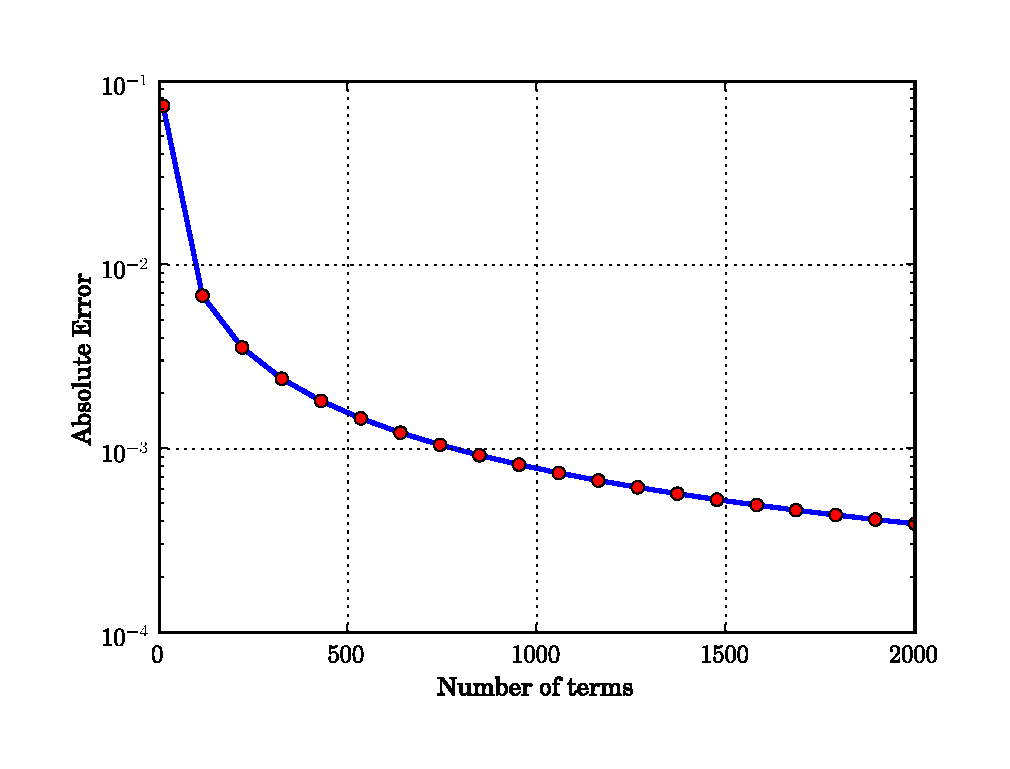
\includegraphics[width=4in]{fig/wallis_pi_convergence}\par\end{centering}


\caption{\label{fig:wallis_pi}Convergence rate for Wallis' infinite product
approximation to $\pi.$}
\end{figure}
\par\end{center}
